\documentclass[aspectratio=169,dvipsnames,table]{beamer}

% Basic packages
\usepackage{hyperref}
% hyperref's un-configured default can draw a visible border box around
% clickable text in some PDF viewers -- hide those borders entirely
% (hidelinks): this deck's link text is already styled deliberately
% (\abrirNoSoftware, \DemoSlide) and a colored border would just add
% noise. Also fills in the PDF's Subject/Keywords, which \title/\author
% derive but the metadata block otherwise leaves blank (checked with
% pdfinfo -- Title/Author were populated, Subject/Keywords empty).
% \ifincludebitnet is set by whichever entry file (apresentacao.tex or
% apresentacao-tese.tex) \input this preamble, before doing so -- see
% their matching comments. Subject/keywords differ per deck, same as
% \title/\subtitle in each entry file.
\ifincludebitnet
\hypersetup{
	hidelinks,
	pdfsubject={As fronteiras da arquitetura de redes neurais: BitNets e redes de pulso},
	pdfkeywords={BitNet, spiking neural networks, quantização, STE, surrogate gradient}
}
\else
\hypersetup{
	hidelinks,
	pdfsubject={Fundamentos computacionais da tese: redes neurais de pulso e lógica paraconsistente},
	pdfkeywords={spiking neural networks, lógica paraconsistente, LIF, surrogate gradient, EEG}
}
\fi

% Absolute position for text and elements
\usepackage[absolute,overlay]{textpos}

% Use latim special characters
\usepackage[utf8]{inputenc}

% DejaVu Sans (Type 1-converted, works under plain pdflatex -- no need for
% xelatex/lualatex) -- the same font the companion software
% (software/efficient_nn_lab) already renders in its matplotlib panels and
% Qt UI, so slides and live software read as one visual system. Sets
% \sfdefault; beamer already routes body text through \sfdefault by
% default, so no \familydefault override is needed.
\usepackage{DejaVuSans}

% Use colors
\usepackage{color}

% Enables graphics
\usepackage{graphicx}

% Better text justification
\usepackage{microtype}

% Enables multicolumn text
\usepackage{multicol}

% Enables \toprule/\midrule/\bottomrule in tables
\usepackage{booktabs}

% Fine-grained control over list spacing (dense two-column slides)
\usepackage{enumitem}
\setlist{itemsep=2pt, topsep=2pt, parsep=0pt}

% Enables math
\usepackage{amsthm}
\usepackage{amsmath}
\usepackage{amssymb}

% Adds some symbols (like slash on a non mathematical context)
\usepackage{textcomp}

% Quote packages, ABNT standard
\usepackage[alf]{abntex2cite}

% Portuguese-specific commands
\usepackage[brazilian]{babel}

% Bibliography
\usepackage[brazilian,hyperpageref]{backref}

% Drawing and plot packages
\usepackage{relsize}
\usepackage{tikz}
\usetikzlibrary{calc}
\usetikzlibrary{positioning}
\usetikzlibrary{decorations.pathreplacing}
\usetikzlibrary{shapes}
\usetikzlibrary{backgrounds}
\usetikzlibrary{patterns}
\usetikzlibrary{fit}
\usetikzlibrary{arrows.meta}

\usepackage{pgfplots}
\usepackage{pgfplotstable}
\pgfplotsset{compat=newest}

% Reuse the thesis' CVD-safe Okabe-Ito palette and diagram semantic roles
% (colors + \tableHeaderRow/\tableZebraStripe) instead of redefining our own.
% visualStyle.tex — Single source of truth for every color used in the
% thesis: tables, the Gantt chart, and TikZ diagrams (images/*.tex).
%
% Palette: Okabe & Ito (2008), "Color Universal Design" — the standard
% categorical palette distinguishable under protanopia, deuteranopia and
% tritanopia. Every color in the thesis must come from here; do not
% \definecolor or use raw color names (fill=orange, fill=green, fill=red, ...)
% ad hoc inside chapters/, tables/*.tex or images/*.tex. Raw xcolor names in
% particular (plain "red"/"green"/"yellow") are NOT CVD-safe — red/green is
% the single most common color-blindness confusion pair.

% ── Okabe-Ito base palette ────────────────────────────────────────────────
\definecolor{cbOrange}{RGB}{230,159,0}
\definecolor{cbSkyBlue}{RGB}{86,180,233}
\definecolor{cbGreen}{RGB}{0,158,115}     % bluish green
\definecolor{cbYellow}{RGB}{240,228,66}
\definecolor{cbBlue}{RGB}{0,114,178}
\definecolor{cbVermillion}{RGB}{213,94,0}
\definecolor{cbPurple}{RGB}{204,121,167}
\definecolor{cbGrey}{RGB}{166,166,166}

% ── Semantic roles (used by every table in the thesis) ───────────────────
% Tint levels below are chosen against two constraints, not eyeballed:
%  1. WCAG 1.4.11 (non-text contrast, >=3:1) / 1.4.3 (text contrast, >=4.5:1)
%     — verified against black text for the band colors below (~9-13:1,
%     comfortably AAA) and against white text for the solid header (~5.2:1,
%     AA). A pale tint (e.g. !35 or lower) still clears contrast but reads
%     as washed-out/grey on paper — the "too dull" failure mode — because
%     contrast alone doesn't capture perceived saturation/vividness.
%  2. Okabe & Ito (2008) hue choices are kept exactly (blue/orange is the
%     most CVD-robust 2-hue pair); only the tint (mix-with-white) percentage
%     is raised for a visibly saturated, "colorful but not extravagant" look.
%
% Header row: solid (untinted) blue background, white bold text.
\colorlet{tableHeaderColor}{cbBlue}
% Zebra striping on long/data-heavy tables: a visible-but-subtle tint of the
% header hue — enough to guide the eye across a row without competing with
% the semantic band colors below. Kept lighter than those on purpose: zebra
% striping is a navigation aid, not information-bearing.
\colorlet{tableAltRowColor}{cbBlue!12}
% Wavelet coefficient examples (tables/{regular,packet}WaveletExample.tex):
% grey = raw signal label, sky blue = row/column index label,
% blue = approximation band (cA), orange = detail band (cD).
% Blue/orange is the single most robust 2-hue pair across all CVD types.
% These ARE information-bearing (which band a cell belongs to), so they are
% tinted much more strongly than the zebra stripe above.
\colorlet{tableSignalLabelColor}{cbGrey}
\colorlet{tableIndexLabelColor}{cbSkyBlue}
\colorlet{tableSignalValuesColor}{cbGreen!55}
\colorlet{tableApproxBandColor}{cbBlue!55}
\colorlet{tableDetailBandColor}{cbOrange!55}

% Gantt chart (chapters/08-proposedApproach.tex, tab:cronogramaGantt):
% same palette, kept here so the chart matches the tables it sits beside.
\colorlet{ganttBarColor}{cbGreen}
\colorlet{ganttMilestoneColor}{cbGreen}
\colorlet{ganttTitleColor}{cbBlue!45}
\colorlet{ganttHighlightColor}{cbOrange}

% ── Reusable header row ────────────────────────────────────────────────────
% Usage inside a tabular/longtable, as the first thing in a header row:
%   \tableHeaderRow \textbf{A} & \textbf{B} \\
\newcommand{\tableHeaderRow}{\rowcolor{tableHeaderColor}\color{white}}

% ── Zebra striping for table/longtable bodies ─────────────────────────────
% Call once, right before \begin{tabular}/\begin{longtable}. Colors rows
% 2, 4, 6, ... (i.e. every data row after a 1-row header) with
% tableAltRowColor; row 1 (the header) is left untouched so \tableHeaderRow
% still controls it. NOTE: \rowcolor itself must always be the literal first
% token of a row — never wrap it in another macro (e.g. a counter-stepper),
% since colortbl's \noalign trick requires nothing to precede it.
\newcommand{\tableZebraStripe}{\rowcolors{2}{white}{tableAltRowColor}}

% ── Wide/wrapping text column, vertically centered ────────────────────────
% Plain p{<width>} columns top-align their content, while ordinary c/l/r
% columns baseline/vertically-center theirs — invisible in a plain \hline
% table, but a visible split (header text sitting below the colored fill)
% once a \rowcolor-filled header row mixes p{} with c/l/r columns. Use the
% column type Y{<width>} instead of p{<width>} in any column spec that will
% share a row with \tableHeaderRow, e.g. \begin{tabular}{@{}Y{10cm}cc@{}}.
\newcolumntype{Y}[1]{>{\raggedright\arraybackslash}m{#1}}

% ── Diagram / flowchart semantic roles (images/*.tex) ─────────────────────
% The thesis has ~20 TikZ flowcharts and node diagrams that all reuse the
% same handful of roles (start/end bubble, process box, decision diamond,
% arrows, autoencoder layer nodes). They used to \definecolor / fill= with
% raw xcolor names (orange, green, yellow, red, gray) independently per
% file — not CVD-safe (plain red/green/yellow is the classic confusion
% triple) and impossible to re-theme consistently. Every images/*.tex file
% must reference these instead of a raw color name.
\colorlet{flowStartEndColor}{cbOrange}
\colorlet{flowProcessColor}{cbGreen}
\colorlet{flowDecisionColor}{cbYellow}
\colorlet{flowArrowColor}{cbGrey}
% Autoencoder-style node diagrams (images/{autoencoder,denoisingAutoencoder,residuo}*.tex):
% grey = input, yellow = hidden/code/latent layer, vermillion = output/reconstruction.
% (Vermillion replaces the original "red" — true red is excluded from the
% Okabe-Ito set for the same red/green confusion reason.)
\colorlet{diagramInputColor}{cbGrey}
\colorlet{diagramHiddenColor}{cbYellow}
\colorlet{diagramOutputColor}{cbVermillion}
% Intermediate/corrupted stage between input and hidden layer (e.g. the
% noised x_hat in images/denoisingAutoencoder.tex, or the pre-activation
% sum in images/residuo.tex) — kept visually distinct from all three roles
% above.
\colorlet{diagramIntermediateColor}{cbSkyBlue}
% Tree diagrams (images/afasias.tex): darker tints so white text keeps
% AA contrast on non-header-sized diagram text.
\colorlet{diagramBranchColor}{cbGreen!80!black}
\colorlet{diagramLeafColor}{cbBlue!80!black}
% Feature-vector pipeline diagrams (images/{bark,mel,linear,lfcc,bfcc}...Vect.tex,
% images/{mel,linear}BandEnergies.tex): single accent color for box/ellipse
% outlines. Okabe-Ito blue, darkened for outline contrast against white fill.
\colorlet{diagramOutlineColor}{cbBlue!80!black}


% Semantic roles for this talk's two "frontiers" -- exact hex values from
% software/efficient_nn_lab/src/efficient_nn_lab/app/theme.py (BITNET_COLOR,
% SNN_COLOR, CONVERGE_COLOR, NEUTRAL_COLOR, ACCENT_COLOR), deliberately
% brighter/more saturated than the thesis' visualStyle.tex tints (those are
% calibrated for AA/AAA contrast in printed text; this talk is projected,
% not printed, and needs to match the live software instead). Do not
% propagate these values back into visualStyle.tex or the thesis chapters.
% bitnetColor/snnColor are darkened just enough (WCAG contrast >=4.5:1 on
% white) to stay legible where motivacao.tex/conclusao.tex use them as
% raw inline \textcolor{...}{} text on the plain white slide background --
% see theme.py's matching comment for the contrast math (same values,
% mirrored). convergeColor/accentColor are never used as raw inline text
% in this deck (only as light !NN!white box-background tints, always
% paired with dark chromeText), so they keep the fully vivid values.
\definecolor{bitnetColor}{HTML}{0073E5}
\definecolor{snnColor}{HTML}{E61F00}
\definecolor{convergeColor}{HTML}{00E38A}
\definecolor{neutralColor}{HTML}{5B6472}
\definecolor{accentColor}{HTML}{FFC300}

% Matches TEXT_COLOR in software/efficient_nn_lab/.../app/theme.py. Used
% as the fixed text color on every colored chrome bar/box below instead
% of white or a hue-matched color: measured contrast ratios (WCAG
% relative-luminance formula) against all five tinted title backgrounds
% range 6.1:1-14.5:1 with near-black text, comfortably clearing the 4.5:1
% AA threshold everywhere. White text only clears >=3:1 (AA-large) on the
% two darkest tints (bitnet/snn) and fails outright on converge/accent/
% neutral; a hue-matched color (e.g. bitnetColor text on a
% bitnetColor!92!white box) is even worse, since text and background
% converge toward the same color -- that was the previous, broken
% behavior in taxonomia.tex/desafios.tex's comparison boxes.
\definecolor{chromeText}{HTML}{111318}

% Packages configuration

\setbeamercolor{background canvas}{bg=}
\setbeamercolor{normal text}{bg=black!20}

% beamer's default "structure" color (a fixed blue) otherwise tints every
% itemize bullet, block title and section number in the deck blue,
% regardless of which of the two frontiers (BitNet=blue, SNN=red,
% convergência=green) is on screen. Pin it neutral so only the frametitle
% bar (set per-section below, in apresentacao.tex, right before each
% \section) and explicit \textcolor{...Color}{} calls carry a hue --
% that is what actually varies the palette across the deck instead of
% bathing everything in blue.
\setbeamercolor{structure}{fg=neutralColor}
\setbeamercolor{title}{fg=chromeText,bg=bitnetColor!92!white}
\setbeamercolor{frametitle}{fg=chromeText,bg=bitnetColor!92!white}

% beamer's default bottom-right navigation icon strip (the little
% arrows/dots cluster) is dead weight for a projected talk -- nobody
% navigates a PDF that way during a presentation, and it adds visual
% noise to all 59 pages. Kill it outright.
\setbeamertemplate{navigation symbols}{}

% Minimal right-aligned page counter so speaker and audience can always
% see "n / total" -- matters for pacing and for Q&A ("volta pro slide do
% STE"). Text is neutralColor on the deck's uniform white frame
% background (sampled from the built PDF: edges are pure white), which
% clears ~6.3:1 WCAG -- same contrast family as chromeText above.
\setbeamertemplate{footline}{%
	\hfill{\scriptsize\color{neutralColor}\insertframenumber{} / \inserttotalframenumber}\hspace{4pt}%
	\vspace{3pt}%
}

% Dedicated (non-dynamic) title-box styles for frames that show two
% frontiers side by side (taxonomia.tex, desafios.tex) -- these must NOT
% follow the per-section frametitle color below, since both colors need
% to be on screen at once.
\setbeamercolor{titleBitnet}{fg=chromeText,bg=bitnetColor!92!white}
\setbeamercolor{titleSnn}{fg=chromeText,bg=snnColor!85!white}
\setbeamercolor{titleConverge}{fg=chromeText,bg=convergeColor!80!white}
\setbeamercolor{titleAccent}{fg=chromeText,bg=accentColor!75!white}

% Clickable "open this demo in the software" cue -- presentation.md phase
% 3/4. #1 = link text (demo name as it appears in the software's sidebar),
% #2 = DemoModule.slug (see software/efficient_nn_lab/src/efficient_nn_lab/
% core/demo.py). "run:" paths resolve against this PDF's own directory, so
% abrir-demo.sh (next to this preamble) does the rest. Many PDF viewers
% block "run:" links by default (see presentation.md 4.2) -- the visible
% text is deliberately also the exact demo name, so it still works as a
% pure navigation label ("go click this in the sidebar") even where the
% link itself does nothing.
\newcommand{\abrirNoSoftware}[2]{%
	\par\vspace{2pt}\noindent%
	{\scriptsize\color{neutralColor}%
		$\blacktriangleright$~\href{run:./abrir-demo.sh #2}{Abrir no software: \textbf{#1}}%
	}%
}

% A full, reserved slide for "now switch to the live software" -- one per
% program section that must be shown (presentation.md phase 3/4, "one
% slide per program section"). Distinct from \abrirNoSoftware, which is
% just a small footer link on a content slide: this is its own frame, so
% during the talk it is an unmissable full-screen cue to alt-tab, not a
% line easy to skip past while still explaining the concept. Reuses the
% "title" beamercolor box (same style as \AtBeginSection's divider), so
% it automatically picks up whichever hue the enclosing \section set --
% no separate color plumbing needed. #1 = demo title (as in the
% software's sidebar), #2 = DemoModule.slug, #3 = one-line presenter cue
% (what to click/say once the software is on screen).
%
% The "run:" link (below) is silently ignored by most PDF viewers
% (presentation.md 4.2), so it cannot be the only way to trigger the demo
% during a talk. Below it, a plain relative shell command is printed in
% monospace so it can be read off and typed, or selected and pasted into
% a terminal already sitting in this .tex file's directory. \path{} (from
% url.sty) was tried first but its verbatim scanner eats the space before
% #2 and wraps the result in "<...>" -- \detokenize{} instead converts
% the already-tokenized argument (slugs use "." and "_", e.g.
% snn.poisson_image) back into plain catcode-12 characters, which
% \texttt{} then typesets like any normal string, space included.
\newcommand{\DemoSlide}[3]{%
	\begin{frame}
		\vfill
		\centering
		\begin{beamercolorbox}[sep=16pt,center,shadow=true,rounded=true]{title}
			{\large\textbf{Demonstração ao vivo}}\\[4pt]
			{\Large #1}
		\end{beamercolorbox}
		\vspace{18pt}
		\href{run:./abrir-demo.sh #2}{\Large $\blacktriangleright$~\textbf{Abrir no software}}
		\vspace{10pt}
		\par{\footnotesize\color{neutralColor} ou, no terminal (a partir desta pasta):}\\[2pt]
		\texttt{\small\detokenize{./abrir-demo.sh }\detokenize{#2}}
		\vspace{18pt}
		\par{\small\color{neutralColor} #3}
		\vfill
	\end{frame}
}

% Enables section slides
\AtBeginSection[]{
	\begin{frame}
		\vfill
		\centering
		\begin{beamercolorbox}[sep=18pt,center,shadow=true,rounded=true]{title}
			\usebeamerfont{title}\insertsectionhead\par
		\end{beamercolorbox}
		\vfill
	\end{frame}
}


\title{As fronteiras da arquitetura de redes neurais}
\subtitle{BitNets e redes de pulso}

\institute{https://github.com/ensismoebius}

\author{André Furlan - ensismoebius@gmail.com}

\date{\the\year}

\begin{document}

	\frame{\titlepage}

	% Frametitle/title bar color changes per section, so the chrome itself
	% signals which frontier is on screen instead of staying blue
	% throughout (see preamble.tex's \setbeamercolor{structure} comment).
	% Must be set BEFORE each \section command: \AtBeginSection's divider
	% frame is emitted during \section's own expansion, so setting the
	% color only after \section would leave the divider frame one step
	% behind.
	\setbeamercolor{title}{fg=chromeText,bg=neutralColor!55!white}
	\setbeamercolor{frametitle}{fg=chromeText,bg=neutralColor!55!white}
	\section{Fundamentos de redes neurais}
		\begin{frame}[shrink]
	\frametitle{Como uma rede neural é construída}
	\framesubtitle{O problema: aprender a transformação em vez de programá-la à mão}
	\small
	\par Dado um sinal de entrada (um pixel, uma amostra de áudio, uma janela de EEG) e a resposta certa que se quer para ele, como chegar da entrada à resposta sem escrever a regra manualmente? A rede neural é essa transformação --- com parâmetros que o próprio treino ajusta, em vez de uma fórmula fixada por quem programou.
	\begin{itemize}
		\item Uma rede neural é organizada em \textbf{camadas}:\newline entrada $\rightarrow$ uma ou mais camadas ocultas $\rightarrow$ saída.\newline
		
		\item Cada neurônio recebe as saídas da camada anterior vezes seus \textbf{pesos} (parte linear), soma tudo, e aplica uma \textbf{ativação} (parte não linear).\newline
		
		
		\item Sem a não linearidade, empilhar camadas equivaleria a uma única camada linear --- é a ativação que dá à rede o poder de aproximar funções complexas.
	\end{itemize}
	\vspace{1pt}
	\begin{center}
		\begin{tikzpicture}[
			node distance=0.75cm,
			neuron/.style={circle, draw=bitnetColor, thick, minimum size=0.4cm},
			lyr/.style={font=\scriptsize\bfseries, text=neutralColor},
			]
			\node[neuron] (x1) at (0,0.8) {};
			\node[neuron] (x2) at (0,0) {};
			\node[neuron] (x3) at (0,-0.8) {};
			\node[neuron] (a) at (2.3,0.55) {};
			\node[neuron] (b) at (2.3,-0.55) {};
			\node[neuron] (c) at (4.6,0.55) {};
			\node[neuron] (d) at (4.6,-0.55) {};
			\node[neuron] (o) at (6.9,0) {};
			\foreach \i in {x1,x2,x3} \foreach \j in {a,b} \draw[-{Latex[length=1.5mm]}, draw=neutralColor!70] (\i) -- (\j);
			\foreach \i in {a,b} \foreach \j in {c,d} \draw[-{Latex[length=1.5mm]}, draw=neutralColor!70] (\i) -- (\j);
			\foreach \i in {c,d} \draw[-{Latex[length=1.5mm]}, draw=neutralColor!70] (\i) -- (o);
			\node[lyr, above=0.15cm of x1] {Entrada (3)};
			\node[lyr, above=0.15cm of a] {Camada 1 (2)};
			\node[lyr, above=0.15cm of c] {Camada 2 (2)};
			\node[lyr, above=0.15cm of o] {Saída (1)};
		\end{tikzpicture}
	\end{center}
\end{frame}

		\DemoSlide{Backpropagation, Rede 3-2-2-1}{backprop.mlp}{}
		\begin{frame}[shrink]
	\frametitle{O que é um peso, e como ele é calculado}
	\small
	\begin{itemize}
		\item Um \textbf{peso} é um número real associado a uma conexão entre dois neurônios --- é o parâmetro que a rede efetivamente \textbf{aprende}. Os dados de entrada não mudam; os pesos, sim.\newline
		
		\item Dentro de um neurônio, os pesos entram na \textbf{combinação linear}: cada entrada é multiplicada pelo seu peso, e os produtos são somados.
	\end{itemize}
	
	\begin{equation*}
		z = \sum_i w_i \, x_i \qquad y = \sigma(z)
	\end{equation*}
	
	\par Exemplo numérico real com o primeiro neurônio da rede do slide anterior:\newline
	\par Entrada $x = [1{,}0,\ 0{,}5,\ -0{,}5]$
	\par Pesos $w = [0{,}4,\ -0{,}3,\ 0{,}6]$.
	
	\begin{equation*}
		z = 0{,}4 \!\cdot\! 1{,}0 + (-0{,}3) \!\cdot\! 0{,}5 + 0{,}6 \!\cdot\! (-0{,}5) = -0{,}05
		\quad\Longrightarrow\quad
		y = \sigma(-0{,}05) \approx 0{,}4875
	\end{equation*}
	
	\par Cada um dos outros neurônios repete exatamente esse cálculo, com sua própria linha de pesos. Antes do treino, os pesos partem de algum valor inicial (aqui, fixos); o que o treino faz é ajustá-los, um pouco a cada passo, para que a saída da rede se aproxime do que se quer.
\end{frame}

		\begin{frame}[shrink]
	\frametitle{Como uma rede neural é treinada}
	\small
	\setlength{\abovedisplayskip}{1pt}
	\setlength{\belowdisplayskip}{1pt}
	\begin{itemize}
		\item \textbf{1. Avanço (Forward)}: calcula a saída $y$ a partir da entrada e dos pesos atuais.
		\item \textbf{2. Perda (loss)}: compara $y$ com o alvo, num único número que cresce com o erro.
		\item \textbf{3. Retropropagação (backward)}: a regra da cadeia calcula $\partial L/\partial w$ --- quanto a perda mudaria se cada peso mudasse um pouco.
		\item \textbf{4. Atualização}: cada peso anda um passo no sentido \textbf{contrário} ao gradiente.
	\end{itemize}
	\begin{equation*}
		w \leftarrow w - \eta \cdot \frac{\partial L}{\partial w}
	\end{equation*}
	\par Exemplo numérico real (neurônio com entrada: $x=2{,}0$, alvo: $=0{,}9$, $w_0=-1{,}0$, $\eta=3{,}0$):
	\begin{equation*}
		\begin{aligned}
			& z = w_0 x = -2{,}0 \Rightarrow \\
			& y = \sigma(z) \approx 0{,}1192 \Rightarrow \\
			& L = \tfrac12(y-\text{alvo})^2 \approx 0{,}3048
		\end{aligned}
	\end{equation*}
	\begin{equation*}
		\frac{\partial L}{\partial w} \approx -0{,}1640
		\quad\Longrightarrow\quad
		w_1 = -1{,}0 - 3{,}0 \cdot(-0{,}1640) \approx -0{,}508
	\end{equation*}
	\par Repetindo os quatro passos, $y$ converge para o alvo. É exatamente esse ciclo que se questiona: E se os pesos só valerem $\{-1,0,1\}$, ou se a ativação virar um pulso discreto?
\end{frame}

		\DemoSlide{Backprop \textrightarrow{} Forward e backward clássicos}{backprop.classic}{}
		\begin{frame}[shrink]
	\frametitle{A camada inteira é uma multiplicação de matrizes}
	\small
	\begin{itemize}
		\setlength{\itemsep}{0pt}
		\item Os slides anteriores calcularam \textbf{um neurônio de cada vez}. Mas a camada toda é \textbf{uma única operação}: empilhe os pesos de cada neurônio como \textbf{linhas} de uma matriz $W$, e o produto escalar de cada neurônio passa a ser uma linha do produto $Wx$.
		\item A regra do mapeamento é toda esta: \textbf{linha} = neurônio de \emph{destino}; \textbf{coluna} = de onde o valor \emph{vem}. Isto é, $W[i,j]$ \emph{é} a seta que liga a entrada $j$ ao neurônio $i$ --- a seta do grafo e a célula da matriz são o mesmo número, não duas representações parecidas.
	\end{itemize}
	\begin{equation*}
		z = W x \qquad y = \sigma(z)
	\end{equation*}
	\par Exemplo numérico real, com a rede da demonstração ($2 \rightarrow 2 \rightarrow 1$):
	\begin{equation*}
		\underbrace{\begin{bmatrix} 0{,}8 & -0{,}4 \\ -0{,}5 & 0{,}9 \end{bmatrix}}_{W_1}
		\underbrace{\begin{bmatrix} 0{,}9 \\ 0{,}4 \end{bmatrix}}_{x}
		=
		\underbrace{\begin{bmatrix} 0{,}56 \\ -0{,}09 \end{bmatrix}}_{z}
		\quad\xrightarrow{\ \sigma\ }\quad
		\underbrace{\begin{bmatrix} 0{,}6365 \\ 0{,}4775 \end{bmatrix}}_{y}
	\end{equation*}
	\par A primeira linha do resultado é $0{,}8 \!\cdot\! 0{,}9 + (-0{,}4) \!\cdot\! 0{,}4 = 0{,}56$: o mesmo $\sum_i w_i x_i$ do slide anterior, agora lido como ``linha vezes vetor''. Já a ativação é um passo \textbf{separado}: $\sigma$ age em cada célula isoladamente, sem misturar linhas --- ao contrário da multiplicação, que existe justamente para combiná-las.
	\vspace{2pt}
	\par\scriptsize\color{neutralColor} Rede menor que a de 4 camadas do começo da seção, de propósito: com matrizes $2\times2$ cada número cabe na tela em corpo legível e cada produto escalar tem só dois termos, então dá para acompanhar \emph{termo a termo} em vez de aceitar o resultado já somado.
	% [SOFTWARE] Backprop -> A rede como matrizes | os mesmos numeros deste
	% slide; um passo por operacao escalar (cada termo, cada soma, cada sigmoide)
	\abrirNoSoftware{Backprop \textrightarrow{} A rede como matrizes}{backprop.matrix}
\end{frame}

		\begin{frame}[shrink]
	\frametitle{O backward é a mesma matriz, transposta}
	\small
	\setlength{\abovedisplayskip}{2pt}
	\setlength{\belowdisplayskip}{2pt}
	\begin{itemize}
		\setlength{\itemsep}{0pt}
		\item No forward, $W_2$ levou 2 valores (os ocultos) para 1 (a saída). O gradiente precisa fazer o caminho \textbf{inverso}: 1 volta para 2. A matriz que faz isso é a \textbf{mesma}, só que transposta: o que era linha vira coluna. \newline \newline \textbf{O erro volta pelos próprios pesos do forward}, não por pesos novos.\newline 
		\item $W \leftarrow W - \eta \, \partial L/\partial W$\newline
	\end{itemize}
	
	\begin{equation*}
		\frac{\partial L}{\partial x} = W^{\top} \frac{\partial L}{\partial z}
		\qquad\qquad
		\frac{\partial L}{\partial W} = \frac{\partial L}{\partial z} \otimes \text{entrada}
	\end{equation*}
	\par A regra da cadeia diluída nessas matrizes é o produto das derivadas locais de cada elo do caminho $x_1 \rightarrow H_1 \rightarrow O \rightarrow L$:
	\begin{equation*}
		\frac{\partial L}{\partial w_{11}} =
		\underbrace{(-0{,}3173)}_{\partial L/\partial y_O} \!\cdot\!
		\underbrace{0{,}2432}_{\sigma'(z_O)} \!\cdot\!
		\underbrace{1{,}2}_{w_{H_1 O}} \!\cdot\!
		\underbrace{0{,}2314}_{\sigma'(z_{H_1})} \!\cdot\!
		\underbrace{0{,}9}_{x_1}
		= -0{,}01928
	\end{equation*}
\end{frame}

		\DemoSlide{Backprop \textrightarrow{} A rede como matrizes}{backprop.matrix}{}
		% Vem depois de fundamentosCadeia.tex de proposito: o slide enuncia a
		% regra da cadeia, e esta demo mostra de qual bloco da rede sai cada
		% fator dela (uma camada = operacao linear + ativacao = dois fatores).
		\DemoSlide{Backprop \textrightarrow{} Camadas e a regra da cadeia}{backprop.chain}{Percorra os passos de $\partial L/\partial a_2$ até $\partial L/\partial b_1$: cada carta é a derivada local de um bloco, na coluna do bloco. Feche com os cinco fatores em fila.}

	\setbeamercolor{title}{fg=chromeText,bg=accentColor!75!white}
	\setbeamercolor{frametitle}{fg=chromeText,bg=accentColor!75!white}
	\section{Motivação}
		\begin{frame}
	\frametitle{O gargalo}
	\only<1>{
		\framesubtitle{Pouca memória muitos dados}
		\begin{itemize}
			\item Redes convencionais (RNAs dedicadas a tarefas de larga escala) crescem em parâmetros muito mais rápido que o poder de processamento dos chips necessitando uma grande quantidade de hardware.\newline
			
			\item Um LLM de 7 bilhões de parâmetros em FP16 ocupa $7\times10^{9}\times 2\text{ bytes} \approx 14\text{ GB}$ \textbf{só para os pesos} --- antes do cache de atenção e das ativações.
			\item Considerando que uma GPU de consumo comum tem 8--24 GB. O modelo não cabe.
		\end{itemize}
	}
	\only<2>{
		\framesubtitle{A implicação}
		\begin{block}{Duas respostas independentes, dois eixos diferentes}
			\begin{itemize}
				\item \textbf{Reduzir quantos bits} descrevem cada peso/ativação $\rightarrow$ \textcolor{bitnetColor}{\textbf{BitNets}}.
				\item \textbf{Reduzir quando/quanto se computa}, processando só em resposta a eventos esparsos $\rightarrow$ \textcolor{snnColor}{\textbf{Redes de pulso}}.
			\end{itemize}
		\end{block}
	}
\end{frame}

		\begin{frame}
	\frametitle{Duas fronteiras, dois eixos ortogonais}
	\small
	\begin{columns}
		\column{.48\linewidth}
		\begin{beamercolorbox}[sep=5pt,rounded=true,shadow=true]{titleBitnet}
			\textbf{Fronteira 1 --- BitNets}
		\end{beamercolorbox}
		\vspace{4pt}
		\par Eixo da \textbf{representação}: quantos bits descrevem cada peso/ativação.
		\begin{itemize}
			\item FP32 $\rightarrow$ FP16 $\rightarrow$ INT8 $\rightarrow$ ternário $\{-1,0,1\}$ $\rightarrow$ binário $\{-1,1\}$.
			\item A rede continua densa e síncrona: \textbf{todo} neurônio ainda computa em \textbf{toda} passada.
			\item O que muda é o \textbf{custo} de cada computação individual.
		\end{itemize}
		\column{.48\linewidth}
		\begin{beamercolorbox}[sep=5pt,rounded=true,shadow=true]{titleSnn}
			\textbf{Fronteira 2 --- Redes de pulso}
		\end{beamercolorbox}
		\vspace{4pt}
		\par Eixo do \textbf{tempo/atividade}: quando e quanto se computa.
		\begin{itemize}
			\item Ativação contínua e síncrona $\rightarrow$ pulso esparso, assíncrono, orientado a evento.
			\item Os pesos podem continuar em precisão plena.
			\item O que muda é \textbf{se} um neurônio computa, a cada instante.
		\end{itemize}
	\end{columns}
	\vspace{2pt}
	\begin{block}{O alvo é o mesmo}
		Ambas atacam o custo (energia, memória, latência) da multiplicação densa em ponto flutuante --- mas por caminhos ortogonais. A \autoref{sec:convergencia} volta a este quadro para mostrar onde as duas se encontram.
	\end{block}
\end{frame}


	\setbeamercolor{title}{fg=chromeText,bg=bitnetColor!92!white}
	\setbeamercolor{frametitle}{fg=chromeText,bg=bitnetColor!92!white}
	\section{Parte I --- BitNets}
		\begin{frame}
	\frametitle{Linha do tempo: da quantização discreta às LLMs de 1 bit}
	\centering
	\resizebox{.94\linewidth}{!}{%
	\begin{tikzpicture}[
		yr/.style={draw=bitnetColor, fill=bitnetColor!15, rounded corners=2pt, minimum height=0.9cm, minimum width=1.6cm, font=\tiny\sffamily, align=center},
		lb/.style={font=\tiny\sffamily, align=center, text width=1.7cm}
		]
		\draw[-{Latex[length=2mm]}, line width=0.6mm, draw=neutralColor] (-0.3,0) -- (12.3,0);

		\node[yr] (n1) at (0,0) {2015};
		\node[lb, below=2pt of n1] {BinaryConnect \cite{courbariaux2016binarized}};

		\node[yr] (n2) at (2.4,0) {2016};
		\node[lb, above=2pt of n2] {BNN \\ XNOR-Net \cite{rastegari2016xnor} \\ TWN \cite{li2016ternary}};

		\node[yr] (n3) at (4.8,0) {2017};
		\node[lb, below=2pt of n3] {TTQ \cite{zhu2017trained}};

		\node[yr] (n4) at (7.2,0) {2022};
		\node[lb, above=2pt of n4] {LLM.int8() \cite{dettmers2022llm}};

		\node[yr] (n5) at (9.6,0) {2023};
		\node[lb, below=2pt of n5] {GPTQ \cite{frantar2023gptq} \\ SmoothQuant \cite{xiao2023smoothquant} \\ BitNet \cite{wang2023bitnet}};

		\node[yr, fill=bitnetColor!45] (n6) at (12,0) {2024};
		\node[lb, above=2pt of n6] {\textbf{BitNet b1.58} \cite{ma2024era}};
	\end{tikzpicture}%
	}
	\begin{itemize}\small
		\setlength{\itemsep}{0pt}
		\item 2015--2017: quantização extrema nasce em \textbf{visão computacional} (redes pequenas, treinadas do zero).
		\item 2022--2023: quantização \textbf{pós-treino} (PTQ) vira estratégia dominante para LLMs já treinados.
		\item 2023--2024: BitNet retoma a ideia de \textbf{treinar do zero} em baixa precisão --- agora em escala de bilhões de parâmetros.
	\end{itemize}
\end{frame}

		\begin{frame}
	\frametitle{Quantizar depois, ou quantizar desde o início?}
	\only<1>{
		\framesubtitle{Dois caminhos, confundidos com frequência}
		\begin{columns}
			\column{.48\linewidth}
			\begin{beamercolorbox}[sep=5pt,rounded=true,shadow=true]{title}
				\textbf{PTQ}: Quantização pós-treino
			\end{beamercolorbox}
			\begin{itemize}
				\item Treina em FP32/FP16 normalmente.
				\item Converte os pesos \textbf{depois}, sem retreinar (ou com pouco ajuste).
				\item Rápido e barato: LLM.int8(), GPTQ, SmoothQuant.
				\item A rede nunca ``viu'' o erro de quantização durante o treino.
			\end{itemize}
			\column{.48\linewidth}
			\begin{beamercolorbox}[sep=5pt,rounded=true,shadow=true]{title}
				\textbf{QAT}: Quantização durante o treino
			\end{beamercolorbox}
			\begin{itemize}
				\item A quantização já ocorre no \textit{forward pass} do treino.
				\item BinaryConnect, BNN, TWN, TTQ, BitNet, BitNet b1.58.
				\item Caro: em geral exige treinar do zero.
				\item A rede se \textbf{adapta} ao erro de quantização.
			\end{itemize}
		\end{columns}
	}
	\only<2>{
		\framesubtitle{PTQ agressiva}
		\small
		\begin{itemize}
			\setlength{\itemsep}{0pt}
			\item Abaixo de $\sim$4 bits, a acurácia de modelos quantizados por PTQ pode cair \textbf{abruptamente} --- não gradualmente.\newline
			
			\item Mecanismo concreto \cite{xiao2023smoothquant}: algumas ativações de LLMs têm \textbf{outliers} --- valores até $100\times$ maiores que o resto do tensor, concentrados em poucos canais.\newline
			
			\item Quando um único fator de escala por tensor precisa cobrir o outlier e os valores normais, os valores normais perdem toda a resolução.\newline
			
			\item Esse é o motivo de existir uma cadeia inteira de métodos de PTQ (LLM.int8(), GPTQ, SmoothQuant) --- cada um mitigando esse efeito de um jeito diferente, em vez de resolvê-lo evitando quantização baixa.
		\end{itemize}
		\begin{alertblock}{Onde o BitNet muda de estratégia}
			Se a rede é treinada \textbf{desde o início} em baixa precisão, ela nunca desenvolve ativações que dependam dessa resolução --- o problema é evitado, não corrigido depois.
		\end{alertblock}
	}
\end{frame}

		\begin{frame}
	\frametitle{A camada BitLinear}
	\only<1>{
		\framesubtitle{Da camada Linear densa à ternária}
		\par Uma camada Linear comum calcula $Y = W X$, com $W$ em FP16/FP32: cada saída soma \textbf{multiplicações reais} entre pesos e ativações contínuos.
		\par O BitNet b1.58 \cite{ma2024era} substitui $W$ por uma versão ternária $\widetilde{W} \in \{-1,0,1\}$, obtida por \textbf{quantização absmean}:
		\begin{equation}
			\gamma = \text{mean}(|W|), \qquad
			\widetilde{W} = \text{round}\big(\text{clip}(W/\gamma,\,-1,\,1)\big)
		\end{equation}
		\par $\gamma$ é um único número por tensor --- guardado à parte para reescalar a saída no fim, não para cada peso individualmente.
	}
	\only<2>{
		\framesubtitle{Exemplo numérico}
		\par Tome três pesos de uma linha de $W$: $w = [0{,}6,\ -0{,}3,\ 0{,}05]$.
		\begin{equation*}
			\gamma = \frac{0{,}6+0{,}3+0{,}05}{3} = 0{,}3056
		\end{equation*}
		\begin{equation*}
			w/\gamma = [1{,}963,\ -0{,}982,\ 0{,}164]
			\xrightarrow{\text{clip}(-1,1)} [1{,}0,\ -0{,}982,\ 0{,}164]
			\xrightarrow{\text{round}} \boxed{[1,\ -1,\ 0]}
		\end{equation*}
		\par O peso original $0{,}05$ (o menor em módulo) \textbf{vira zero} --- é descartado, não aproximado. Os outros dois viram $\pm 1$.
		\par As ativações $X$ recebem seu próprio tratamento, quantização \textbf{absmax} para INT8: $\widetilde{X} = \text{round}(X \cdot 127/\max(|X|))$, com \textit{clip} em $[-128,127]$.
	}
	\only<3>{
		\framesubtitle{O que essa troca compra}
		\begin{itemize}
			\item Com $\widetilde{W} \in \{-1,0,1\}$, a multiplicação $\widetilde{W}\cdot\widetilde{X}$ vira: \textbf{some} $\widetilde{X}$ (peso $+1$), \textbf{subtraia} $\widetilde{X}$ (peso $-1$), ou \textbf{ignore} (peso $0$).
			\item Nenhuma multiplicação real acontece no lado dos pesos --- só somas/subtrações de inteiros, mais um único rescalonamento por $\gamma$ ao final.
			\item É exatamente a operação mais cara da tabela de energia vista na motivação ($\sim$3,7 pJ por multiplicação FP32) que desaparece --- trocada por somas de $\sim$0,03 pJ, repetidas em bilhões de operações por inferência.
		\end{itemize}
	}
\end{frame}

		\DemoSlide{BitNet \textrightarrow{} Quantização}{bitnet.quant}{}
		\DemoSlide{BitNet \textrightarrow{} Forward}{bitnet.forward}{}
		\begin{frame}[shrink]
	\frametitle{Treinar através de uma função que não tem gradiente}
	\small
	\begin{itemize}
		\item $\text{round}(\cdot)$ e $\text{clip}(\cdot)$ são \textbf{funções em degrau}: a derivada é zero em quase todo ponto, e indefinida nos degraus.
		\item Retropropagação padrão não tem o que propagar através delas --- o gradiente morre.
	\end{itemize}
	\vspace{1pt}
	\begin{block}{A solução: \textit{Straight-Through Estimator} (STE)}
		\begin{itemize}
			\item \textbf{Forward}: usa os pesos quantizados $\widetilde{W}$ normalmente.
			\item \textbf{Backward}: finge que a quantização foi a função identidade --- deixa o gradiente passar direto para uma cópia dos pesos em precisão plena, mantida ``nos bastidores'' e só quantizada de novo a cada passada.
		\end{itemize}
	\end{block}
	\vspace{0pt}
	\begin{alertblock}{Ponte com a Parte II}
		É a \textbf{mesma} ideia por trás do \textit{gradiente substituto} em redes de pulso \cite{eshraghian2023training}: forward com a função em degrau real, backward com uma aproximação suave, diferenciável. Duas subáreas, independentemente, chegaram à mesma solução para o mesmo problema estrutural.
	\end{alertblock}
	% [SOFTWARE] BitNet -> Backward -> STE | checkpoint final (derivada
	% real vs. constante 1 do STE)
	\abrirNoSoftware{BitNet \textrightarrow{} Backward \textrightarrow{} STE}{bitnet.ste}
	% [SOFTWARE] BitNet -> Exemplo guiado | demo bonus, se sobrar tempo: o ciclo
	% completo forward->perda->STE->update num peso so (presentation.md, secao 3)
	\abrirNoSoftware{BitNet \textrightarrow{} Exemplo guiado (bônus)}{bitnet.guided}
	\vspace{-3pt}
\end{frame}

		\DemoSlide{BitNet \textrightarrow{} Backward \textrightarrow{} STE}{bitnet.ste}{}
		% Demo de reserva. Estava como \abrirNoSoftware no rodape de
		% bitnetTreinamento.tex; aquele quadro ja usa [shrink] e os links
		% foram removidos de la, o que deixou esta demo sem nenhuma porta
		% de entrada no PDF (test_every_demo_is_reachable_from_the_lecture_deck).
		% Como quadro proprio nao disputa espaco com nada.
		\DemoSlide{BitNet \textrightarrow{} Exemplo guiado (bônus)}{bitnet.guided}{Ciclo completo forward \textrightarrow{} perda \textrightarrow{} STE \textrightarrow{} update num peso só: peso latente 0,80 \textrightarrow{} 0,84. Demo de reserva, se sobrar tempo.}
		\begin{frame}
	\frametitle{BitNet b1.58: o que 1,58 bit compra}
	\framesubtitle{Comparado a LLaMA em FP16, mesmo tamanho de modelo \cite{ma2024era}}
	\begin{center}
		\begin{tabular}{lcc}
			\toprule
			& \textbf{3B parâmetros} & \textbf{70B parâmetros} \\
			\midrule
			Memória de GPU & $3{,}55\times$ menor & $7{,}2\times$ menor \\
			Velocidade de decodificação & $2{,}71\times$ mais rápido & $4{,}1\times$ mais rápido \\
			\textit{Throughput} & --- & $8{,}9\times$ maior \\
			Perplexidade / tarefas finais & \multicolumn{2}{c}{equivalente ao FP16} \\
			\bottomrule
		\end{tabular}
	\end{center}
	\vspace{8pt}
	\begin{itemize}
		\item ``Equivalente'' aqui não é aproximação --- os autores reportam paridade estatística com a linha de base FP16 a partir de $\sim$3B parâmetros.
		\item \alert{Abaixo dessa escala, a paridade some}: em modelos pequenos, a capacidade perdida pela quantização ternária pesa mais do que o modelo consegue compensar.
		\item De onde vem o nome ``1,58 bit'': $\log_2(3) \approx 1{,}58$ --- o número de bits necessário para representar 3 estados ($-1,0,1$) por peso.
	\end{itemize}
\end{frame}

		\begin{frame}
	\frametitle{Hardware e limitações}
	\begin{columns}
		\column{.5\linewidth}
		\begin{beamercolorbox}[sep=5pt,rounded=true,shadow=true]{title}
			A promessa de hardware
		\end{beamercolorbox}
		\begin{itemize}
			\item Sem pesos em ponto flutuante, não há necessidade de multiplicadores de ponto flutuante --- só somadores de inteiros.
			\item Abre espaço para ASICs dedicados, mais simples e mais eficientes por operação.
		\end{itemize}
		\column{.5\linewidth}
		\begin{beamercolorbox}[sep=5pt,rounded=true,shadow=true]{title}
			Os limites atuais
		\end{beamercolorbox}
		\begin{itemize}
			\item Kernels/\textit{runtimes} para pesos ternários ainda são imaturos em GPUs convencionais, otimizadas para INT8/FP16 denso.
			\item Exige treinar do zero: não há como converter um checkpoint FP16 já treinado com a mesma qualidade.
			\item Ganho de paridade só aparece a partir de $\sim$3B parâmetros.
		\end{itemize}
	\end{columns}
\end{frame}


	\setbeamercolor{title}{fg=chromeText,bg=snnColor!85!white}
	\setbeamercolor{frametitle}{fg=chromeText,bg=snnColor!85!white}
	\section{Parte II --- Redes de pulso}
		\begin{frame}
	\frametitle{Redes neurais de pulso (RNP)}
	\only<1>{
		\framesubtitle{Por que pulsos?}
		\begin{itemize}
			\item Uma RNA convencional ativa \textbf{todos} os neurônios em \textbf{toda} passada --- o custo energético não depende do conteúdo do dado, só do tamanho da rede.\newline
			
			\item O neurônio biológico só dispara quando o potencial acumulado ultrapassa um limiar; fica quieto o resto do tempo.\newline
			
			\item Maass (1997) chamou as RNPs de \textit{"modelos de redes neurais \textbf{terceira geração}"} \cite{maass1997networks} --- depois do perceptron (1ª geração) e das redes com ativação contínua/sigmoide (2ª geração).
		\end{itemize}
	}
	\only<2>{
		\framesubtitle{Uma ressalva importante}
		\par Uma RNP \textbf{não} é uma simulação um-para-um de neurônios biológicos. Ela aproxima certas capacidades computacionais de propriedades biológicas específicas --- não o neurônio inteiro.\newline
		
		\par Modelos mais fiéis à biologia existem (Hodgkin--Huxley \cite{gerstner2014neuronal}, dendritos não-lineares), mas são caros demais para treinar em escala. As RNPs usadas em aprendizado de máquina adotam modelos simplificados, como o \textbf{LIF} (próximo slide).
	}
\end{frame}

		\begin{frame}[shrink]
	\frametitle{RNA vs. RNP: o par que se confunde}
	\small
	\begin{columns}
		\column{.48\linewidth}
		\begin{beamercolorbox}[sep=5pt,rounded=true,shadow=true]{title}
			Rede Neural Artificial (RNA)
		\end{beamercolorbox}
		\begin{itemize}
			\item Ativação: valor \textbf{contínuo} por neurônio, por camada.
			\item Processamento \textbf{síncrono}: uma passada completa por amostra.
			\item Sem dimensão temporal intrínseca (a menos que seja recorrente).
			\item Custo computacional fixo, independente da atividade.
		\end{itemize}
		\column{.48\linewidth}
		\begin{beamercolorbox}[sep=5pt,rounded=true,shadow=true]{title}
			Rede Neural de Pulso (RNP)
		\end{beamercolorbox}
		\begin{itemize}
			\item Ativação: \textbf{pulso} (0 ou 1), esparso no tempo.
			\item Processamento \textbf{orientado a evento}: só computa quando há pulso.
			\item Dinâmica temporal \textbf{intrínseca}: potencial de membrana acumula ao longo do tempo.
			\item Informação codificada em \textbf{taxa} e/ou \textbf{tempo} de disparo \cite{kasabov2019time}.
		\end{itemize}
	\end{columns}
	\vspace{2pt}
	\begin{alertblock}{Consequência prática}
		Uma RNP processa naturalmente \textbf{fluxos} de dados (áudio, EEG, eventos de câmera) --- mas processar um único dado estático exige ``esticá-lo'' ao longo de vários passos de tempo, um custo que a RNA não tem.
	\end{alertblock}
	% [SOFTWARE] SNN -> Sinal e spikes | Play uma vez (cruzamento de
	% nivel vira spike discreto)
	\abrirNoSoftware{SNN -> Sinal e spikes}{snn.spikes}
	% [SOFTWARE] SNN -> Codificacao Poisson | mesmo sinal, spikes
	% probabilisticos (contraste com a demo acima)
	\abrirNoSoftware{SNN -> Codificação Poisson}{snn.poisson}
\end{frame}

		\DemoSlide{SNN \textrightarrow{} Normalização: por característica x por janela}{snn.normalization}{Áudio padroniza cada característica com média/desvio ajustados uma vez no treino (CMVN); EEG recalcula a cada janela, e uma deriva de +50~$\mu$V some. Só o caminho ajustado pode vazar dados de teste -- em silêncio.}
		\DemoSlide{SNN \textrightarrow{} Sinal e spikes}{snn.spikes}{}
		\DemoSlide{SNN \textrightarrow{} Codificação Poisson}{snn.poisson}{}
		\DemoSlide{SNN \textrightarrow{} Ruído estrutural da codificação}{snn.encoding_noise}{"Direta > latência > Poisson" pode ser só o chão de ruído estrutural de cada codificação, não uma diferença real de informação.}
		\DemoSlide{SNN \textrightarrow{} Perda incompatível com a codificação}{snn.encoding_loss_mismatch}{Perda de contagem sobre latência: o treino reporta perda zero sem corrigir nada. Perda certa (SpikeTimeLoss): uma unidade que nunca dispara fica sem gradiente. Duas falhas silenciosas -- e a validação que as torna barulhentas.}
		\begin{frame}
	\frametitle{O neurônio \textit{Leaky Integrate-and-Fire} (LIF)}
	\only<1>{
		\framesubtitle{O modelo RC}
		\begin{columns}
			\column{.60\linewidth}
			\begin{itemize}
				\item O LIF se comporta como um circuito Resistor-Capacitor (RC).
				\item $R$: resistência de vazamento; $C$: capacitância; $V_{mem}$: potencial acumulado; $\vartheta$: interruptor que descarrega o capacitor (dispara um pulso) ao atingir o limiar.
				\item Governado por \cite{eshraghian2023training}:
				
				
				 $\tau\frac{dV_{mem}}{dt} = R\,I_{in}(t) - V_{mem}(t)$, com $\tau = R\cdot C$ .
			\end{itemize}
			\column{.40\linewidth}
			\begin{center}
				\includegraphics[width=.85\linewidth]{../../00-thesis/monography/images/rcmodel}\par
				{\tiny Fonte: \cite{eshraghian2023training}}
			\end{center}
		\end{columns}
	}
	\only<2>{
		\framesubtitle{Exemplo numérico: decaimento sem entrada}
		\par Sem corrente ($I_{in}=0$), a equação do slide anterior vira $\tau\,dV_{mem}/dt = -V_{mem}$. Separando as variáveis e integrando os dois lados:
		\begin{equation*}
			\begin{aligned}
				\frac{dV_{mem}}{V_{mem}} = -\frac{dt}{\tau}
				\ & \Rightarrow\
				\int \frac{dV_{mem}}{V_{mem}} = \int -\frac{dt}{\tau}
				\ \Rightarrow\
				\ln V_{mem} = -\frac{t}{\tau} + k \\
				& \Rightarrow\ V_{mem}(t) = e^{k}\cdot e^{-t/\tau}
				\ \Rightarrow\
				V_{mem}(t) = V_{mem}(0)\cdot e^{-t/\tau}
			\end{aligned}
		\end{equation*}
		\par {\small (pois em $t=0$: $e^{k}=V_{mem}(0)$)}
		\par Com $R=5\,\Omega$, $C=1\,F$ (logo $\tau = R\cdot C = 5$) e potencial inicial $V_{mem}(0)=1$:
		\begin{equation*}
			V_{mem}(1) = 1 \cdot e^{-1/5} \approx 0{,}8187
		\end{equation*}
		\par O potencial \textbf{vaza} exponencialmente na ausência de estímulo --- daí o nome \textit{leaky}. Quando um estímulo chega, o potencial sobe (mesma matemática, sinal oposto) até cruzar um limiar $V_{th}$, disparando um pulso e reiniciando.
	}
	\only<3>{
		\framesubtitle{Comportamento completo simulado}
		\begin{center}
			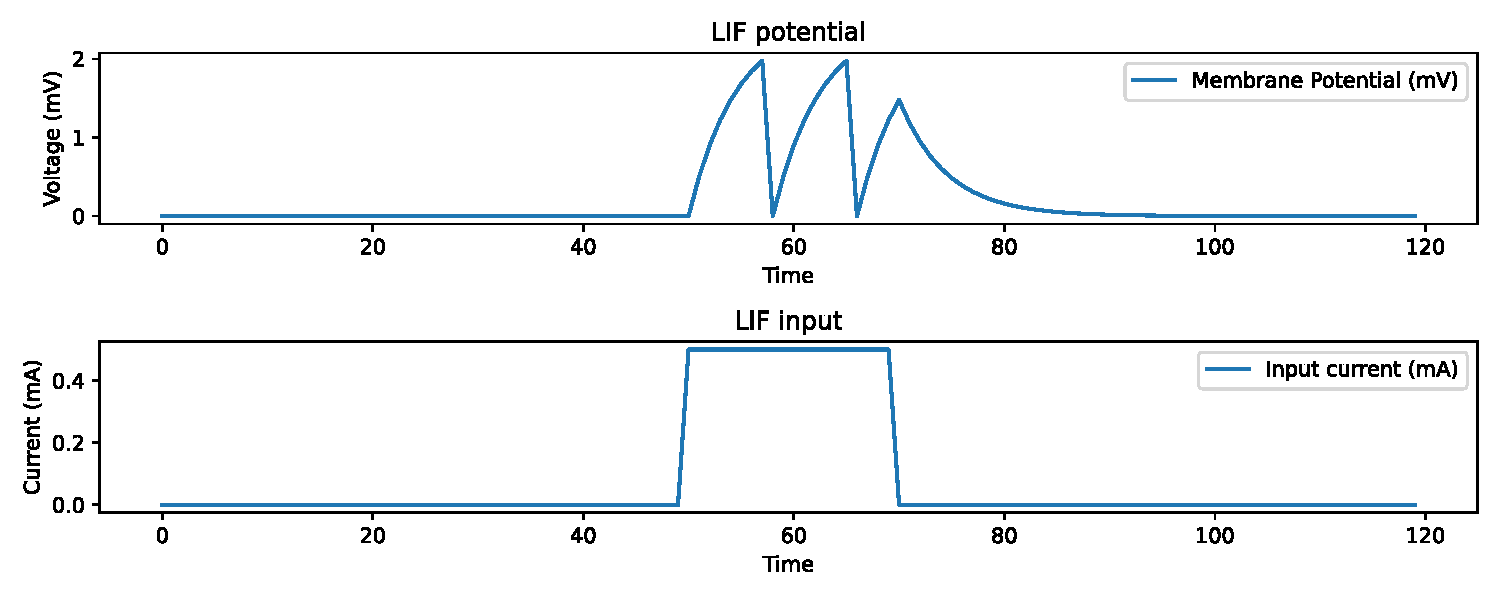
\includegraphics[width=1\linewidth]{../../00-thesis/monography/images/membranePotentialFull}\par
			{\tiny Corrente de 0,5 mA injetada entre os passos 51 e 70. Fonte: elaborado pelo autor.}
		\end{center}
	}
\end{frame}

		\DemoSlide{SNN \textrightarrow{} LIF}{snn.lif}{Os parâmetros padrão (tau=5, R=5, V\_th=1) já reproduzem o exemplo numérico anterior; aperte Play para o comportamento completo.}
		\DemoSlide{SNN \textrightarrow{} time\_steps x delta\_t}{snn.timesteps}{Quantos quadros x quanto dura um quadro -- e por que a ordem das linhas no tensor (T*B,F) importa.}
		\begin{frame}
	\frametitle{Esparsidade: onde mora a eficiência}
	\only<1>{
		\begin{columns}
			\column{.55\linewidth}
			\begin{center}
				\includegraphics[height=6.0cm]{../../00-thesis/monography/images/sparsity}\par
				{\tiny Eixo horizontal: tempo. Eixo vertical: índice do neurônio. Fonte: elaborado pelo autor.}
			\end{center}
			\column{.42\linewidth}
			\small
			\begin{itemize}
				\item Na maior parte do tempo, a \textbf{grande maioria} dos neurônios está silenciosa.
				\item Pulsos são representados como \textbf{uns} dispersamente distribuídos em uma sequência de \textbf{zeros} \cite{eshraghian2023training}.
				\item Um neurônio LIF bem parametrizado tolera ruído: age como um \textbf{filtro passa-baixa}, só disparando quando o sinal se acumula de forma sustentada.
			\end{itemize}
		\end{columns}
	}
	\only<2>{
		\begin{alertblock}{A promessa, com precisão}
			Esparsidade só vira economia de energia real em hardware que sabe \textbf{pular} o zero. Em GPU/TPU convencional, a esparsidade é invisível ao hardware --- ele computa a multiplicação por zero do mesmo jeito.
		\end{alertblock}
		\vspace{4pt}
		\par Volta-se a este ponto na próxima seção, sobre hardware neuromórfico.
	}
\end{frame}

		\DemoSlide{SNN \textrightarrow{} Codificação Poisson (imagem)}{snn.poisson_image}{}
		\begin{frame}
	\frametitle{Como treinar uma função que não tem gradiente?}
	\only<1>{
		\framesubtitle{\ifincludebitnet O mesmo problema estrutural do BitNet\else Quatro famílias de resposta, historicamente\fi}
		\footnotesize
		\par A função de disparo do LIF se aproxima de uma \textbf{função em degrau} (Heaviside): dispara ou não dispara, sem meio-termo. Sua derivada é zero em quase todo ponto --- a descida de gradiente padrão não tem o que propagar \cite{kasabov2019time}.
		\par Quatro famílias de resposta, historicamente:
		\begin{itemize}
			\setlength{\itemsep}{0pt}
			\item \textbf{STDP}: regra local --- se o neurônio pré-sináptico dispara \textbf{antes} do pós-sináptico, a conexão se fortalece; se depois, se enfraquece. Biologicamente plausível, não supervisionada.
			\item \textbf{Gradiente substituto + BPTT}: usa a função em degrau real no \textit{forward}, e uma aproximação suave e diferenciável só no \textit{backward}\ifincludebitnet{} --- a mesma lógica do STE do BitNet\fi.
			\item \textbf{Algoritmos evolutivos}: seleção dos hiperparâmetros mais aptos ao longo de gerações.
			\item \textbf{Reservatório / computação dinâmica}: treina só a camada de saída, mantendo pesos recorrentes fixos (\textit{echo state networks}, \textit{liquid state machines}).
		\end{itemize}
	}
	\only<2>{
		\framesubtitle{Alternativa: converter em vez de treinar}
		\begin{itemize}
			\item Treina uma \textbf{RNA convencional}, com técnicas padrão de otimização.
			\item \textbf{Converte} os pesos treinados para uma RNP, balanceando pesos e limiares de disparo \cite{diehl2015fast, rueckauer2017conversion}.
			\item Evita o problema do gradiente por completo --- mas herda limitações: geralmente precisa de \textbf{mais passos de tempo} para aproximar a acurácia da RNA original, e nem toda arquitetura converte bem.
		\end{itemize}
	}
\end{frame}

		\DemoSlide{SNN \textrightarrow{} Surrogate gradient}{snn.surrogate}{Percorra os checkpoints "A derivada real" até "O gradiente substituto".}
		\DemoSlide{SNN \textrightarrow{} Normalização dependente de limiar (tdBN)}{snn.tdbn}{BatchNorm comum fixa variância 1 e, com V\_th = 2, cala a camada; tdBN espalha a corrente em $\alpha \cdot V_{th}$, e a fração acima do limiar deixa de depender de V\_th.}
		\DemoSlide{SNN \textrightarrow{} Regularização de taxa de disparo}{snn.firing_rate_reg}{Um neurônio quase morto e um em rajada são empurrados de volta à faixa alvo de taxa de disparo; dentro da faixa, a penalidade não faz nada.}
		\begin{frame}
	\frametitle{Retropropagação através do tempo (BPTT): o que é?}
	\framesubtitle{Estendendo a descida de gradiente para redes com dinâmica e memória}
	\small
	\par Em redes convencionais \textit{feedforward}, a informação viaja apenas de camada em camada ($l \to l+1$), sem memória de estados passados.
	\par Em uma SNN, cada neurônio LIF acumula potencial de membrana $u_t$ (equivalente discreto do potencial $V_{mem}(t)$) que evolui ao longo de $T$ passos temporais:
	\begin{itemize}
		\item A resposta no passo atual $t$ depende diretamente do que aconteceu nos passos anteriores.
		\item Se a rede erra em $t=T$, o erro pode ter sido causado por um pulso disparado lá atrás em $t=1$.
	\end{itemize}
	\par A \textbf{Retropropagação através do tempo} (\textit{Backpropagation Through Time} --- BPTT) calcula o gradiente do erro retrocedendo \textbf{entre as camadas e através dos passos de tempo}.
	\begin{block}{Por que ela é necessária?}
		Sem o BPTT, a rede não aprende atribuição de crédito temporal (\textit{temporal credit assignment}): treinar cada passo isoladamente apagaria a memória da dinâmica de membrana.
	\end{block}
\end{frame}

\begin{frame}
	\frametitle{BPTT: a intuição temporal}
	\framesubtitle{Um neurônio vê um filme, não uma foto isolada}
	\small
	\par Exemplo com neurônio LIF: potencial $u_t = \beta\,u_{t-1} + x_t$ (onde $\beta=0{,}5$ é o decaimento e $x_t$ a entrada no instante $t$), limiar $V_{th}=1{,}0$ e reset para $0$ após disparo:
	\begin{center}
		\footnotesize
		\begin{tabular}{ccccc}
			\toprule
			\textbf{Passo $t$} & \textbf{Entrada $x_t$} & \textbf{Dinâmica $u_t$} & \textbf{$u_t \ge 1{,}0$?} & \textbf{Pulso?} \\
			\midrule
			1 & $0{,}8$ & $0{,}5(0) + 0{,}8 = 0{,}8$ & Não & Não \\
			2 & $0{,}0$ & $0{,}5(0{,}8) + 0 = 0{,}4$ & Não & Não (decaimento retido) \\
			3 & $0{,}8$ & $0{,}5(0{,}4) + 0{,}8 = 1{,}0$ & \textbf{Sim} & \textbf{Sim} (dispara e reseta) \\
			\bottomrule
		\end{tabular}
	\end{center}
	\begin{block}{A dependência temporal na prática}
		O pulso em $t=3$ só ocorreu porque o estímulo de $t=1$ ainda estava retido na memória da membrana no passo 2! Sem $x_1$, $u_3$ seria apenas $0{,}8$ (sem disparo).
	\end{block}
	\begin{itemize}
		\item Para ajustar os pesos corretamente, o gradiente do erro em $t=3$ precisa viajar no tempo até $t=1$.
	\end{itemize}
\end{frame}

\begin{frame}
	\frametitle{BPTT: abrir a rede ao longo do tempo (\textit{Unrolling})}
	\framesubtitle{Transformando recorrência temporal em camadas equivalentes}
	\small
	\par Para calcular o gradiente no tempo, a rede é "desenrolada" conceitualmente em $T$ passos temporais:
	\begin{center}
		\begin{tikzpicture}[>=Stealth, every node/.style={font=\small}]
			\tikzset{
				rede/.style={draw, rounded corners, thick, text width=2.4cm,
					minimum height=1.3cm, inner sep=5pt, align=center, fill=snnColor!8},
				entrada/.style={font=\normalsize},
				saida/.style={font=\normalsize}
			}
			\node[rede] (r1) at (0,0) {\textbf{Rede}\\camadas + LIF};
			\node[rede] (r2) at (4.8,0) {\textbf{Rede}\\camadas + LIF};
			\node[rede] (r3) at (9.6,0) {\textbf{Rede}\\camadas + LIF};
			\node[entrada] (x1) at (0,1.05) {$x_1$};
			\node[entrada] (x2) at (4.8,1.05) {$x_2$};
			\node[entrada] (x3) at (9.6,1.05) {$x_3$};
			\node[saida] (s1) at (0,-1.0) {$s_1$};
			\node[saida] (s2) at (4.8,-1.0) {$s_2$};
			\node[saida] (s3) at (9.6,-1.0) {$s_3$};
			\node[font=\footnotesize, text=neutralColor] at (4.8,1.7) {Mesma rede, pesos compartilhados $W$, desenrolada em 3 instantes};
			\draw[->,thick] (x1) -- (r1);
			\draw[->,thick] (x2) -- (r2);
			\draw[->,thick] (x3) -- (r3);
			\draw[->,thick] (r1) -- (s1);
			\draw[->,thick] (r2) -- (s2);
			\draw[->,thick] (r3) -- (s3);
			\draw[->,thick,snnColor] (r1.east) -- node[above, midway, font=\scriptsize, yshift=1pt] {estado $h_1$} (r2.west);
			\draw[->,thick,snnColor] (r2.east) -- node[above, midway, font=\scriptsize, yshift=1pt] {estado $h_2$} (r3.west);
		\end{tikzpicture}
	\end{center}
	\begin{itemize}
		\item Cada bloco executa um passo temporal: $x_t$ é a entrada, $s_t \in \{0,1\}$ é o pulso emitido e $h_t$ é o estado interno de membrana entregue ao passo seguinte.
		\item \textbf{Pesos compartilhados}: Todas as réplicas temporais utilizam rigorosamente os mesmos pesos $W$.
	\end{itemize}
\end{frame}

\begin{frame}[shrink]
	\frametitle{BPTT: o caminho retrógrado do erro}
	\framesubtitle{Propagação do gradiente no espaço e no tempo}
	\small
	\par No \textit{forward}, o tempo avança de $t=1$ até $T$. No \textit{backward}, a regra da cadeia percorre o grafo no sentido inverso:
	\begin{center}
		\begin{tikzpicture}[>=Stealth, every node/.style={font=\small}]
			\tikzset{passo/.style={draw, rounded corners, thick, minimum width=2.1cm,
				minimum height=0.75cm, align=center, fill=snnColor!8}}
			\node[passo] (p1) at (0,0) {Passo $t=1$};
			\node[passo] (p2) at (3.0,0) {Passo $t=2$};
			\node[passo] (p3) at (6.0,0) {Passo $t=3$};
			\draw[->,thick] (p1) -- node[above, font=\footnotesize] {$h_1$} (p2);
			\draw[->,thick] (p2) -- node[above, font=\footnotesize] {$h_2$} (p3);
			\node (loss) at (7.8,0) {$L(s_3)$};
			\draw[->,thick] (p3.east) -- (loss.west);
			\draw[->,thick,snnColor] (6.0,-0.65) -- (0,-0.65);
			\node[font=\footnotesize, text=snnColor] at (3.0,-0.92)
				{Gradiente temporal retorna: $t = 3 \longrightarrow 2 \longrightarrow 1$};
		\end{tikzpicture}
	\end{center}
	\begin{itemize}
		\setlength{\itemsep}{1pt}
		\item \textbf{Acumulação nos pesos}: Como $W$ atua em todo $t$, a atualização total $\frac{\partial L}{\partial W}$ soma os gradientes locais $\frac{\partial L}{\partial W^{(t)}}$ de cada instante:
		\vspace{-2pt}\[
			\frac{\partial L}{\partial W} = \sum_{t=1}^{T} \frac{\partial L}{\partial W^{(t)}}
		\]\vspace{-2pt}
		\item \textbf{A ponte com o Gradiente Substituto}: Como a derivada do degrau de disparo é zero, o BPTT usa o \textbf{gradiente substituto} para fornecer uma derivada suave que permita ao erro atravessar o pulso \cite{wu2018spatio, eshraghian2023training}.
	\end{itemize}
\end{frame}

\begin{frame}[shrink]
	\frametitle{BPTT: o mesmo exemplo, agora com números}
	\framesubtitle{$\partial L/\partial W$ passo a passo, continuando o exemplo da intuição temporal}
	\small
	\par Retomando o exemplo anterior, com peso de entrada $W$: $u_t = \beta\,u_{t-1} + W x_t$, com $\beta=0{,}5$, $W=1$ e vetor de entradas $x=(0{,}8;\ 0;\ 0{,}8)$ --- mesma dinâmica: $u_1=0{,}8$, $u_2=0{,}4$, $u_3=1{,}0$. Com perda quadrática $L=\tfrac12(u_3-u_{\mathrm{alvo}})^2$ e alvo $u_{\mathrm{alvo}}=0{,}9$: o erro final é $\partial L/\partial u_3 = u_3-u_{\mathrm{alvo}} = 0{,}1$.
	\begin{center}
		\footnotesize
		\begin{tabular}{cccc}
			\toprule
			\textbf{Passo $t$} & \textbf{$\partial u_3/\partial u_t = \beta^{3-t}$} & \textbf{$x_t$} & \textbf{Contribuição $\frac{\partial L}{\partial u_3}\cdot\frac{\partial u_3}{\partial u_t}\cdot x_t$} \\
			\midrule
			1 & $\beta^2 = 0{,}25$ & $0{,}8$ & $0{,}1 \times 0{,}25 \times 0{,}8 = 0{,}02$ \\
			2 & $\beta^1 = 0{,}50$ & $0$ & $0{,}1 \times 0{,}50 \times 0 = 0$ \\
			3 & $\beta^0 = 1{,}00$ & $0{,}8$ & $0{,}1 \times 1{,}00 \times 0{,}8 = 0{,}08$ \\
			\bottomrule
		\end{tabular}
	\end{center}
	\begin{equation*}
		\frac{\partial L}{\partial W} = \sum_{t=1}^{3} \frac{\partial L}{\partial u_3}\cdot\frac{\partial u_3}{\partial u_t}\cdot x_t = 0{,}02 + 0 + 0{,}08 = 0{,}10
	\end{equation*}
	\par O termo $t{=}1$ \textbf{ainda contribui} ($0{,}02$) dois passos antes do erro: é essa soma que faz o aprendizado "olhar para trás" no tempo. Já $t{=}2$ contribui \textbf{zero}, não pela distância, mas porque $x_2=0$: sem entrada, não há informação sobre $W$.
\end{frame}

\begin{frame}
	\frametitle{Retropropagação através do tempo (BPTT): qual a sua importância?}
	\framesubtitle{Equivalência com Deep Learning moderno e desafios de memória}
	\small
	\begin{itemize}
		\item \textbf{Importância científica e prática}:
		\begin{itemize}
			\item Unificou o treino de SNNs com a infraestrutura de diferenciação automática (PyTorch, JAX).
			\item Superou regras heurísticas locais, permitindo aprendizado supervisionado de ponta a ponta.
		\end{itemize}
	\end{itemize}
	\begin{center}
		\footnotesize
		\begin{tabular}{lcc}
			\toprule
			& \textbf{Rede feedforward} & \textbf{SNN + BPTT} \\
			\midrule
			\textbf{Caminho do erro} & Apenas entre camadas & Entre camadas \textbf{e no tempo} \\
			\textbf{Estados retidos} & Ativações estáticas & Histórico $u_t$ em todo $t \in [1, T]$ \\
			\textbf{Memória na GPU} & $O(\text{profundidade})$ & $O(\text{profundidade} \cdot T)$ \\
			\bottomrule
		\end{tabular}
	\end{center}
	\begin{itemize}
		\item \textbf{Desafio prático}: Janelas longas elevam a memória. Solução: BPTT Truncado (TBPTT) \cite{eshraghian2023training}.
	\end{itemize}
	\par\vfill{\tiny Referências: \cite{wu2018spatio, eshraghian2023training}.}
\end{frame}

		\label{sec:snnHardware}
		\begin{frame}
	\frametitle{Hardware neuromórfico}
	\begin{itemize}
		\item \textbf{TrueNorth} (IBM, 2014): 1 milhão de neurônios, chip totalmente assíncrono e orientado a evento \cite{merolla2014truenorth}.
		\item \textbf{Loihi} (Intel, 2018): aprendizado \textit{on-chip}, arquitetura \textit{manycore} orientada a evento \cite{davies2018loihi}.
		\item \textbf{SpiNNaker} (Manchester, 2014): milhões de núcleos ARM emulando pulsos em tempo real biológico \cite{furber2014spinnaker}.
	\end{itemize}
	\vspace{8pt}
	\begin{alertblock}{O modo de falha silencioso}
		O ganho energético de uma RNP só se realiza \textbf{nesse hardware especializado}. Rodada em GPU/TPU convencional --- otimizada para multiplicação densa, não para pular zeros --- simular $T$ passos de tempo por amostra pode deixar a RNP \textbf{mais lenta} que a RNA equivalente. Esparsidade sem hardware que saiba explorá-la é só um número bonito no papel.
	\end{alertblock}
\end{frame}

		\begin{frame}
	\frametitle{Aplicações e redes de pulso + \textit{transformers}}
	\begin{itemize}
		\item \textbf{Câmeras de eventos} (DVS): sensores que já emitem pulsos nativamente --- casamento direto com RNPs.
		\item \textbf{EEG/BCI}: sinais biológicos já são fluxos temporais esparsos por natureza --- domínio onde a codificação temporal da RNP é vantagem, não custo extra.
		\item \textbf{Computação de borda}: dispositivos vestíveis e embarcados, onde bateria é o recurso mais escasso.
		\item \textbf{Spikformer} \cite{zhou2023spikformer}: reformula o mecanismo de atenção do \textit{transformer} em operações compatíveis com pulsos, aproximando as duas linhagens de arquitetura que dominam \textit{deep learning} hoje.
	\end{itemize}
	\vspace{8pt}
	\par Panorama mais amplo do campo em \cite{roy2019towards}.
\end{frame}


	\setbeamercolor{title}{fg=chromeText,bg=convergeColor!80!white}
	\setbeamercolor{frametitle}{fg=chromeText,bg=convergeColor!80!white}
	\section{Convergência}
		\label{sec:convergencia}
		\begin{frame}
	\frametitle{Onde as duas fronteiras se encontram}
	\centering
	\resizebox{!}{4.3cm}{%
	\begin{tikzpicture}[
		quad/.style={draw=neutralColor, minimum width=4.6cm, minimum height=3cm, align=center, font=\small},
		axislbl/.style={font=\small\sffamily, align=center}
		]
		% Quadrant fills
		\node[quad, fill=neutralColor!12] (bl) at (0,0) {\textbf{RNA padrão}\\[2pt]\footnotesize FP32/FP16, densa,\\ síncrona};
		\node[quad, fill=bitnetColor!18] (br) at (4.8,0) {\textbf{BitNet / BNN / TWN}\\[2pt]\footnotesize binário/ternário, mas\\ ainda densa e síncrona};
		\node[quad, fill=snnColor!18] (tl) at (0,3.2) {\textbf{RNP de precisão plena}\\[2pt]\footnotesize pesos FP32,\\ esparsa e orientada a evento};
		\node[quad, fill=convergeColor!25] (tr) at (4.8,3.2) {\textbf{RNP quantizada}\\[2pt]\footnotesize binário/ternário \emph{e}\\ esparsa/orientada a evento};

		% Axes
		\draw[-{Latex[length=2mm]}, draw=neutralColor!70] (-2.7,-1.6) -- (7.5,-1.6);
		\node[axislbl] at (2.4,-2.05) {precisão dos pesos: alta $\longrightarrow$ ternária/binária};
		\draw[-{Latex[length=2mm]}, draw=neutralColor!70] (-2.7,-1.6) -- (-2.7,4.8);
		\node[axislbl, rotate=90] at (-3.15,1.6) {denso/síncrono $\longrightarrow$ esparso/evento};
	\end{tikzpicture}%
	}
	\vspace{2pt}
	\begin{itemize}\small
		\item Um pulso já \textbf{é}, por definição, um valor binário no tempo (disparou ou não) --- a RNP é quantização extrema no eixo \textbf{temporal}, assim como o BitNet é quantização extrema no eixo dos \textbf{pesos}.
		\item O quadrante superior direito --- RNPs com pesos binários/ternários --- é direção de pesquisa \textbf{emergente}, ainda sem método canônico consolidado.
	\end{itemize}
	% [SOFTWARE] Comparacao -> ANN x BitNet x SNN | ultimo checkpoint
	% (tabela completa)
	\abrirNoSoftware{Comparação \textrightarrow{} ANN x BitNet x SNN}{comparison}
\end{frame}

		\DemoSlide{Comparação \textrightarrow{} ANN x BitNet x SNN}{comparison}{Avance até o último checkpoint: a tabela completa ANN x BitNet x SNN.}
		\DemoSlide{Comparação \textrightarrow{} Autoencoders (SNN x LSTM x GRU x Transformer)}{comparison.autoencoders}{Como o Meeting01 compara quatro famílias sem trapacear: mesmo gargalo, mesmo alvo, referências média e PCA. A PCA é real (janelas sintéticas); as famílias ficam sem números inventados -- só o experimento LOSO os preenche.}
		% Lógica paraconsistente (tese de doutorado do autor): uma métrica
		% geométrica (alpha/beta -> plano paraconsistente -> D_penalized) que
		% ranqueia QUALIDADE de um resultado antes de treinar qualquer coisa --
		% usada pela tese para ranquear extratores de features, e reutilizada
		% pelo experimento paraconsistentGA do software/nn (fora da monografia)
		% como objetivo de uma busca NSGA-II por arquiteturas. Cabe em
		% "Convergência": é literalmente o ponto onde a lógica de ranqueamento
		% da tese encontra a busca de arquitetura.
		\DemoSlide{Paraconsistente \textrightarrow{} Plano paraconsistente}{paraconsistent.plane}{Alpha (compacidade intraclasse) e beta (sobreposição interclasse) definem um ponto no plano, com quatro cantos: Verdade, Falsidade, Ambiguidade, Indefinição.}
		\DemoSlide{Paraconsistente \textrightarrow{} D\_truth x D\_penalized}{paraconsistent.dpenalized}{Por D\_truth, um extrator "morto" ($\sqrt{2} \approx 1{,}41$) passa à frente de um fraco porém real (1,50); D\_penalized leva os três cantos ruins a exatamente 2 e fecha essa brecha -- contribuição central da tese do autor.}
		\DemoSlide{Paraconsistente \textrightarrow{} Busca genética de arquiteturas (extensão)}{paraconsistent.ga_pareto}{Fora da monografia: o paraconsistentGA do software/nn usa D\_penalized como objetivo de uma busca NSGA-II -- dominância, fronteira de Pareto, teto de latência pela regra de Deb, e um cardápio, não um vencedor.}
		\begin{frame}
	\frametitle{O tema comum}
	\begin{itemize}
		\item Ambas as fronteiras abandonam a \textbf{multiplicação densa em ponto flutuante} como operação fundamental --- uma pela via da \textbf{representação} (menos bits por peso), outra pela via do \textbf{tempo} (menos ativações por passo).
		\item As duas nasceram de comunidades diferentes (compressão de modelos vs. neurociência computacional) e, de forma independente, chegaram à mesma solução estrutural para treinar através de uma função não-diferenciável: o STE do BitNet e o gradiente substituto da RNP são o mesmo truque.
		\item O mesmo gargalo de fundo motiva as duas: energia dominada por \textbf{movimento de dado}, não por operações aritméticas em si --- a tabela de energia vista na abertura desta palestra.
	\end{itemize}
\end{frame}


	\setbeamercolor{title}{fg=chromeText,bg=accentColor!75!white}
	\setbeamercolor{frametitle}{fg=chromeText,bg=accentColor!75!white}
	\section{Desafios e síntese}
		\begin{frame}
	\frametitle{Desafios abertos}
	\small
	\begin{columns}
		\column{.48\linewidth}
		\begin{beamercolorbox}[sep=5pt,rounded=true,shadow=true]{titleBitnet}
			\textbf{BitNets}
		\end{beamercolorbox}
		\begin{itemize}
			\setlength{\itemsep}{0pt}
			\item Ecossistema de \textit{kernels}/hardware ainda imaturo.
			\item Exige treinar do zero --- não reaproveita checkpoints existentes.
			\item Paridade com FP16 só a partir de $\sim$3B parâmetros.
		\end{itemize}
		\column{.48\linewidth}
		\begin{beamercolorbox}[sep=5pt,rounded=true,shadow=true]{titleSnn}
			\textbf{Redes de pulso}
		\end{beamercolorbox}
		\begin{itemize}
			\setlength{\itemsep}{0pt}
			\item \textit{Gap} de acurácia em tarefas complexas frente a RNAs grandes.
			\item Sobrecarga de simular $T$ passos em hardware convencional.
			\item Fragmentação entre \textit{frameworks} (snnTorch, SpikingJelly, Lava).
		\end{itemize}
	\end{columns}

	\begin{alertblock}{Convergência}
		Co-projeto algoritmo-hardware ainda é incipiente para as duas frentes \textbf{separadamente} --- combiná-las (RNP quantizada) multiplica essa dificuldade em vez de somá-la.
	\end{alertblock}
\end{frame}

		\begin{frame}
	\frametitle{Síntese}
	\begin{itemize}
		\item Duas respostas independentes à mesma pressão: o custo energético e de memória do paradigma denso em ponto flutuante.
		\item \textcolor{bitnetColor}{\textbf{BitNets}} atacam a \textbf{representação} --- quantos bits descrevem cada peso.
		\item \textcolor{snnColor}{\textbf{Redes de pulso}} atacam o \textbf{tempo/atividade} --- quando vale a pena computar.
		\item O ganho real de ambas depende de hardware co-desenhado para explorá-las --- sem isso, permanecem truques de compressão em vez de mudanças de paradigma.
	\end{itemize}
\end{frame}


	\begin{frame}[allowframebreaks]
		\frametitle{Referências}
		\bibliography{referencias.bib}
	\end{frame}

\end{document}
